\section{Experimental Evaluation}
\label{sec:evaluation}

This experimental evaluation will answer the following questions:
\begin{itemize}
\item What is the effectiveness of \MP{}? (Section~\ref{sec:effectiveness}) 	
\item What is the performance overhead of \MP{}? (Section~\ref{sec:perf})
\item What is the memory overhead of \MP{}? (Section~\ref{sec:memory})
\end{itemize}

Experiments were performed on a two-processor machine, where each processor is Intel(R) Xeon(R) Gold 6230 and each processor has 20 cores. This machine has 256GB of main memory, 20MB of L2 cache, and 1280KB L1 cache. The underlying OS is Ubuntu 18.04.3 LTS, installed with the Linux-5.3.0-40. All applications were compiled using GCC-7.5.0, with \texttt{-O2} and \texttt{-g} flags.

\subsection{Effectiveness}
\label{sec:effectiveness}

In order to evaluate the effectiveness, we evaluate \MP{} with five widely-used allocators, including two versions of the Linux allocator (version 2.21 and 2.28), TCMalloc~\citep{tcmalloc}, jemalloc, and Hoard, and two secure allocators, i.e. DieHarder and OpenBSD. These allocators include both sequential and BiBOP-style allocators. Secure allocators were included, since they have their unique memory management policies. 

For the evaluation, we use the default configurations of these allocators. However, we make some changes in order to  intercept synchronizations. Since Linux allocators are included in \texttt{glibc} libraries, they invoke the internal synchronizations (\texttt{lll\_lock}) directly, which cannot be intercepted by \MP{}. They are recompiled separately as a stand-alone library. Because Hoard is using \texttt{std::lock\_guard} for its synchronization, we replaced them with POSIX spin locks to track its synchronization behavior.

%\todo{Let's use a table to list all dramatic difference between these allocators. This gives us some evidence of allocators}
%\subsection{Issues Identified in Different Allocators}

\begin{comment}

\begin{table}[h]
  \centering
  \caption{Abnormal metrics of allocators for different applications.\label{table:abnormal}}
  \footnotesize
  \setlength{\tabcolsep}{0.2em}
\begin{tabular}{l | l | l | l | l}
\hline
Applications & Allocator & Behavior & Abnormal Metrics & Root Cause \\ \hline
cache-thrash & TcMalloc & $47.7\times$ slowdown & Contention rate for PFS lines: 50\% & Root Cause \RN{1} \\ \hline
dedup & glibc-2.21 & 20\% slowdown &  \# of Madvise for small allocations: & Root Cause \RN{2} \\ \hline
freqmine & jemalloc &  Memory consumption & memory blowup: 2174230K (37\%) & Root Cause \RN{3} \\ 
 & &  & external fragmentation: 1132045K (19\%) \\ \hline
swaptions  &  DieHarder  & $9\times$ slowdown  & 
	Small reused alloc: 377476 cycles 	& Root Cause \RN{4} \\
& & & Small free: 331745 cycles, and 4.9 cache misses & \\ 
& & & Per-lock acquisition: 353448 cycles & \\\cline{4-5}
& & & External fragmentation: 1878K(37\%) & Root Cause \RN{5} \\
& & & cache utilization 55\%, page utilization 35\% & \\\cline{2-5}
& Hoard & $6.3\times$ slowdown & 
	Small reused alloc: 68933 cycles, 9.4 cache misses 	& Root Cause \RN{6} \\
	
& & & Small free: 53402 cycles, 11.8 cache misses & \\ 
& & & 1.54 locks per-operation & \\
\cline{4-5}
& & & Memory blowup: 4789K( 81\%) & Root Cause \RN{7} \\
& & & cache utilization 62\%, page utilization 51\% & \\\cline{2-5}
& OpenBSD & $8\times$ slowdown & Small re-used alloc: 98962 cycles, 4.5 cache misses & Root Cause \RN{8}\\ 
& & & Small free: 101081 cycles, 7 cache misses & \\ 
& & & 1.1 locks per-operation &  \\ \hline
  \end{tabular}
\end{table}
\end{comment}


%issues of allocators that were detected by \MP{}.
%The detailed data reported by \MP{} will be presented in order to show the helpfulness of its report. 

\paragraph{TcMalloc:}
%TcMalloc typically performs very well in almost all applications, except \texttt{cache-thrash} and  \texttt{cache-scratch}. For instance,
TcMalloc runs $38\times$ slower than the default allocator for \texttt{cache-scratch}. \MP{} reports the runtime of allocations and deallocations of TcMalloc, which is at a normal range. But it reports around a 22\% cache invalidation rate for passive false sharing issues, which is the major reason causing the significant slowdown.  
%TcMalloc actually experiences both active and passive false sharing issues. For active false sharing, TcMalloc will get one object for a thread from its central heap each time, so that two continuous objects can be utilized by two different threads. Since 
Based on our understanding, TcMalloc always places a freed object to the current thread's per-thread cache, which may introduce passive false sharing that two objects in the same cache line are accessing by different threads. 
%In comparison, the Linux allocator always returns an object back to its original arena, avoiding passive false sharing.  
%TcMalloc also has 8\% internal fragmentation and 8\% external fragmentation for \texttt{swaptions}, which explains that why it has more memory overhead than other allocators. 

\paragraph{glibc-2.21:}  For \texttt{dedup}, glibc-2.21 has a known bug that may invoke excessively large number of \texttt{madvise} systems calls under certain memory use patterns~\cite{madvise}. \MP{} reports 505241 \texttt{madvise} invocations in 8.6 seconds, and the runtime of each \texttt{madvise} is about $12266$ cycles (much higher than the normal one). \texttt{madvise} introduce high kernel contention with page faults and memory-related system calls. Changing the threshold of shrink\_heap reduces the runtime from 8.6 seconds to 6.9 seconds (with 20\% improvement).

%\MP{} also reports 52\% memory wastes caused by memory blowup for this application. That helps explain why glibc-2.21 are using 740 MB more memory than TcMalloc.  

%\paragraph{jemalloc:} jemalloc typically has good performance, but has a greater memory consumption caused by both memory blowup and external fragmentation. For \texttt{freqmine} application, jemalloc has 43\% memory wastes caused by blowup. That helps explain that why it consumes 40\% more memory than TcMalloc, and 38\% more than glibc-2.21. In comparison, TcMalloc only has 2\% memory wastes and glibc-2.21 has 7\% memory wastes.  

\paragraph{DieHarder:} DieHarder runs $5.75\times$ slower than the default Linux allocator for \texttt{swaptions}. This application reflects multiple design issues of DieHarder. First, \MP{} reports an abnormally high amount of cache misses for each deallocation (around 112). Based on our investigation, DieHarder checks all miniheaps to identify the original location of an object, which introduces multiple cache misses due to the checking on multiple miniheaps. Second, \MP{} reports that DieHarder has one lock acquisition per allocation and five lock acquisitions per free operation, with 44\%  and 47\% lock contention rate for small and big allocations. The data helps explain that  DieHarder utilizes a global lock, which is certainly not scalable.  

%\textit{Root Cause \RN{5}}: we also notice that DieHarder introduces external fragmentation, around 37\%. As described before, this also includes the size of skipped objects, which is caused by DieHarder's over-provision allocation mechanism. Since DieHarder will also randomly choose some objects, that is maybe the cause of its low cache utilization and page utilization. 


\paragraph{Hoard:} 
For \texttt{swaptions}, \texttt{Hoard} is running around $2.07\times$ slower than the default allocator. \MP{} reports abnormal lock information related with medium-size objects (between 256 bytes and 8K bytes): it acquires 1.9 locks per new allocation, 1.73 locks per re-used allocation, and 2.73 locks per free operation. 
%These operations also incur 14\%, 18\% and 14\% lock contention separately. In addition to that, \MP{} reports that the average cycles of each lock is more than 400 cycles, which is much more than 30~70 cycles for the serial phase. 
Multiple locks per operation is caused by Hoard's hash mechanism: ``we use a simple hash function to map thread id’s to per-processor heaps....., there is not a one-to-one correspondence between threads and processors''~\cite{Hoard}. Because multiple threads can be mapped to the same heap, Hoard has to introduce a lock to protect each heap, which is different from TcMalloc and jemalloc's per-thread buffer. 

In addition to that, \MP{} further reports abnormal lock contention rate for some locks, up to 87\% for new allocations and 47\% for re-used allocations in parallel phase. Therefore, we utilized the debugger to identify the reason: Hoard has a threshold (defined in hoardThresholdFunctionClass) for returning a super-block back into the global pool of super-blocks based on the emptyness. Unfortunately, one deallocation could cause the current super-block to be placed into the global pool, while the next allocation will move the super-block back to the thread-local buffer. That is, the back-and-forth of moving the super-block introduces high contention on the lock of protecting the super-block pool. We changed the threshold from 64K to 4K to reduce the migration, where this single change improves the runtime from 26.17 seconds to 12.76 seconds. \textit{This is a new bug that is never reported elsewhere}. 

%Also, its overhead of using many levels of templates cannot completely go away, since Hoard has a lot of code like this: SmallHeap::malloc(), or getHeap().malloc(), Heap::malloc(). Based on our evaluation on an application (canneal) with a big number of allocations, the allocation cycles for a new allocation for Hoard will be around 520 cycles, which is 2.8X of TcMalloc (180 cycles). The cycles for a re-used allocation will be 187 cycles, which is 2.3X times of TcMalloc (83 cycles). The number of instructions is also multiple times more than TcMalloc.

%Hoard also has 40\% memory wastes for \texttt{swaptions}, where 26\% is from its external fragmentation.  
 
%\paragraph{OpenBSD:} \textit{Root Cause \RN{8}:}  OpenBSD has $8\times$ slowdown for \texttt{swaptions}, comparing to the default allocator. Based on its report, we find out that OpenBSD has the similar issue as Hoard, since it acquires more than one lock for each operation. By checking the code, we find out that OpenBSD has the same global lock for all allocations and deallocations, which is the possible reason for its big slowdown. Also, OpenBSD also has a big cache misses for its re-used allocations and deallocations for small objects, which is possibly another reason why it has a big slowdown. For OpenBSD, we also observe that it has significant big number of instructions than other allocators, which as 430 instructions for deallocating a small object, and 295 instructions for a re-used allocation. This is possibly another reason for its big slowdown. 

%\paragraph{jemalloc:}
%During evaluation, the \texttt{reverse\_index} benchmark was found to perform approximately 21\% slower when paired with \texttt{jemalloc} versus the default Linux allocator. Upon inspection, we find that, with \texttt{jemalloc}, the program exhibited over $2x$ the number of CPU cycles associated with the deallocation execution path, as well as a 34\% increase in critical section duration (i.e., the cycles spent within outermost critical sections).




 
\begin{comment}
\renewcommand{\arraystretch}{1.5}
\begin{table}[!ht]
  \centering
   \caption{Important   Metrics\label{tab:metrics}}
  
    \begin{tabular}{l|l|l|l}
    \hline
\multirow{5}{*} {Performance} & \multirow{3}{*}{Allocation Runtime} & New Allocation  (Small) & 80\\ \cline{3-4}
& & Reallocation  (Small) & 1000 \\ \cline{3-4}
& &  Large Allocation & 1000 \\ \cline{2-4}
& \multirow{2}{*}{Deallocation Runtime} & Small  &  \\ \cline{3-4}
& & Large & 100 \\ \cline{1-4}
    
    \end{tabular}
\end{table}
	
\end{comment}

\subsubsection{Observations for Allocators:} 

We have some observations on commonalities of a performant allocator. 

\paragraph{Synchronization:} It is better to reduce lock usages for an allocator. For instance, TcMalloc and jemalloc utilize per-thread cache to store objects, so that there is no need to acquire a lock if an allocation can be satisfied from a per-thread heap. Hoard, although with its per-thread heap design, actually can be slowed down a lot via its hashing mechanism. The other two counterexamples are OpenBSD's allocator and DieHarder. They both use the same lock to manage different size classes, which is one most important issue for their big slowdown. 

\paragraph{Active/Passive False Sharing:} TcMalloc although with the good performance, but it has very serious both active and passive false sharing. This could significantly slowdown the performance, even if it has almost the fast allocation/deallocation speed.  

\paragraph{Cache Misses:} Some allocators, such as DieHarder, Hoard, and  OpenBSD, have multiple cache misses per operation. That could sometime be the reason for their slowdown. The opposite for them is TcMalloc and jemalloc that always have fewer cache misses. We believe that this issue can be reduced with a better design, such as with better metadata design.  

\paragraph{Kernel space synchronization:} Kernel contention is actually very common based on our evaluation. We could observe this from the runtime of memory related system calls.  However, it is sometimes difficult to evaluate its potential impact.

\paragraph{Fine-grained size:} The Linux allocator is the only allocator has very fine-grained size, where two continuous size classes only have the difference of 16 bytes. This mechanism may impose less internal fragmentation. However, it will has the issue of external fragmentation. Although the Linux allocator also can coalesce and split objects to reduce internal fragmentation, it will pay some additional performance cost. That is the reason why the Linux allocator is typically slower than TcMalloc for most applications.

\paragraph{Re-used allocations and deallocations of small objects:} Based on our observation these two aspects are the most important to the  performance of applications, due to its large number. This is also the fast path, which should have less conflicts and fewer instructions.  


%For a performant allocator, what's the common things within the average allocator. We could utilize a table to list the average points of each allocator. Potentially, we could utilize these parameters to evaluate a new allocator. 

%For evaluating purpose, we could provide two information, one is the average with all evaluated allocators, another one is to omit one allocator with the lowest scores. 


%It seems that BIBOP style allocators are the trend of allocators, which not only has a better performance overhead on average, but also has better safety by separating the metadata from the actual heap. 



\subsection{Performance Overhead}
\label{sec:perf}

\begin{figure}[!ht]
\centering
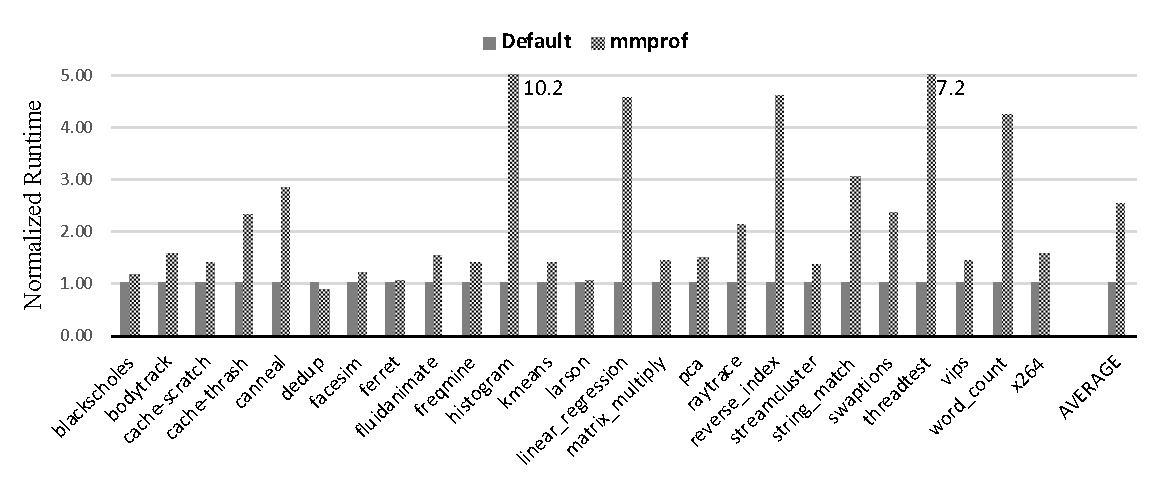
\includegraphics[width=5.5in]{figures/perfoverhead}
\caption{Performance overhead of \texttt{mmprof}, normalized to the runtime of default Linux allocator.\label{fig:overhead}}
\end{figure}

We evaluate the performance overhead of 
\MP{} using PARSEC~\citep{parsec},  Phoenix~\citep{phoenix}, and synthetic applications from Hoard~\cite{Hoard}. The performance overhead can be seen in Figure~\ref{fig:overhead}, which is the average runtime of five executions. From this figure, we can see that \MP{} runs $2.6\times$ slower than the default allocator, where two applications (\texttt{histogram} and \texttt{threadtest}) impose over $5\times$ performance overhead. Based on our understanding, both the number of memory operations and the number of lock acquisitions can significantly impact the performance overhead. To help the explanation, we further collect the characteristics of these applications, as shown in Table~\ref{table:characteristics}.  

First, if an application invokes extensive applications and deallocations in a short period of time, then \MP{} may introduce a large performance overhead. For each memory operation, \MP{} invokes two RDTSC instructions to collect the runtime, updates multiple counters, and updates the state in the global hash table. Second, the number of lock acquisitions inside memory operations could also significantly affect the performance. Similarly, \MP{} also collects the runtime data of each lock acquisition via the RDTSC instruction, and update different counters. 
Since \texttt{canneal} invokes 11 million memory operations and 0.3 million locks acquisitions per second, and \texttt{threadtest} has 6 million memory operations and 33 lock acquisitions per second, that explains why these applications have a large overhead with \MP{}.  

\texttt{histogram} and \texttt{linear\_regression} are two exceptions, since they have a small number of allocations. For these two applications, \texttt{histogram}'s execution time is 0.12 seconds and  \texttt{linear\_regression} is 0.3 seconds.  \MP{} has an initialization phase to perform the initialization, and an finalization phase to analyze the data and write out results to the external file, which may add more overhead than a program's execution time. 
%For instance, \texttt{histogram} only takes 0.12 seconds to finish. Therefore, \MP{} adds more overhead than the program's execution time.  has the same issue, with the total execution time of 0.3 seconds.  
%for some tiny applications like \texttt{histogram}, which only takes 0.1 second when running along, \MP{}'s initialization and conclusion would take more time than themselves. Thus, performance overhead ratios for tiny applications could be larger.
%\texttt{threadtest} actually imposes more performance overhead, due to the reason that most memory opeations are actually 



%some applications invoke allocations intensively and almost simultaneously from different threads, \MP{} may introduce more contention in the hash table when checking every object's status, and higher contention rates would cause programs' slowdown.
\begin{comment}
For example, according to \ref{sec:memory}, 
canneal 2.86x   11438194.73 (alloc+free)/sec    42282925 alloc+free 311044.69 lockacqs/sec
reverse_index 4.59x 973245.43 (alloc+free)/sec 40000387 alloc+free 120407.33 lockacqs/sec
threadtest 7.21x 6 228 715.40 (alloc+free)/sec 256000203 alloc+free 33 239 532.98 lockacqs/sec



For example, according to \ref{sec:memory}, 
linear_regression 4.56x, 0.3s when running alone, 2 alloc+free
word_count 4.26x, 1.71s when running alone, 481 alloc
histogram 10.23x, 0.12s when running alone, 4 alloc+free

Upon every allocation and deallocation, \MP{} collects the runtime and acquisition information.

\end{comment}

\begin{table}[h]
  \centering
  \footnotesize
  \setlength{\tabcolsep}{0.2em}
\begin{tabular}{l|c|r|r|r|r}
\hline
\multicolumn{1}{c|}{Application} & 
\multicolumn{1}{c|}{Runtime}    & 
\multicolumn{1}{c|}{New Alloc}     & 
\multicolumn{1}{c|}{Reused Alloc}     & 
\multicolumn{1} {c|}{Free}     & 
\multicolumn{1}{c}{Lock Acqs} \\ \hline
  blackscholes & 16.7 & 8 & 1 & 7 & 11 \\ \hline   
   bodytrack & 8.5 & 20150 & 460616 & 480765 & 871397 \\ \hline    
   cache-scratch & 3.0 & 44 & 400000 & 400043 & 47 \\ \hline    
   cache-thrash  & 2.4 & 43 & 3999960 & 4000002 & 45\\ \hline  
   canneal & 29.4 & 8756242 & 12385221 & 21141462 & 9144714 \\ \hline    
   dedup & 12.7 & 3384984 & 683368 & 1750378 & 4864027 \\ \hline    
   facesim & 159.2 & 953143 & 3955049 & 4094483 & 1678963 \\ \hline    
   ferret & 25.3 & 149680 & 236867 & 415914 & 417370\\ \hline    
   fluidanimate & 12.3 & 229912 & 1 & 229913 & 307124 \\ \hline    
   freqmine & 20.2 & 1810 & 4 & 1070 & 15926 \\ \hline    
   histogram & 0.12 & 2 & 0 & 2 & 3 \\ \hline    
   kmeans & 16.4 & 200691 & 533 & 200579 & 303705 \\ \hline    
   larson & 15.1 & 2408955 & 33726797 & 36095750 & 38088835 \\ \hline   
   linear\_regression & 0.3 & 1 & 0 & 1 & 2 \\ \hline    
   matrix\_multiply & 4.8 & 83 & 0 & 82 & 85 \\ \hline    
   pca & 9.2 & 16131 & 29 & 72 & 16466 \\ \hline    
   raytrace & 41.1 & 5000115 & 15000100 & 20000172 & 5000240 \\ \hline   
   reverse\_index & 1.5 & 1632810 & 106173 & 1738982 & 1806110\\ \hline  
   streamcluster & 23.5 & 47 & 8798 & 8844 & 17622\\ \hline    
   string\_match & 0.6 & 8 & 0 & 7 & 10 \\ \hline    
   swaptions & 14.5 & 2040 & 47999756 & 48000385 & 48002039\\ \hline    
   threadtest & 7.7 & 1280122 & 126720000 & 128000081 & 255944404\\ \hline    
   vips 6.5 & 8128 & 1420072 & 1428019 & 1526404\\ \hline    
   word\_count & 1.7 & 481 & 0 & 0 & 481\\ \hline   
   x264 & 24.2 & 10 & 0 & 9 & 13\\ \hline    \hline 
   \hline
  \end{tabular}
  \caption{Characteristics of applications\label{table:characteristics}}
\end{table}
\subsection{Memory Overhead}
\label{sec:memory}
To evaluate the memory consumption, we  evaluate \MP{} with glibc-2.28. In total, the memory consumption with \MP{} is around $2.6\times$ more than that without \MP{}, where the specific data is skipped due to the page limitation. 
%Overall, the memory overhead for applications with large footprint is typically smaller, comparing to applications with small footprint. 

 Multiple reasons may contribute to \MP{}'s memory overhead. First, \MP{} adds a hash table to store all allocated objects, in order to differentiate new and re-used allocations, which adds significant memory overhead. Second, \MP{} maintains per-page information to track memory usage and measure page utilization rate, and per-cacheline information to measure cache utilization rate. 
 %Third, \MP{} stores per-thread counters for each size class, including the counters for internal fragmentation and active allocations, which will reduce the contention caused by using the global counters by trading the memory overhead for the performance. 

%For instance, \MP{} imposes around $2.6\times$ memory overhead for \texttt{canneal}, due to 8.7 million new allocations. 
 

%In total, \MP{} introduces 53.6\% memory overhead. It has different behaviors for applications with large footprint (with the original memory consumption larger than 100 MB) and with small footprint. The average memory overhead for applications with large footprint is 179\%, but it is $45\times$ for small footprint applications. For instance, for \texttt{freqmine} and \texttt{linear\_regression}, \MP{} only adds $68.1\%$ and $2.3\%$ separately. 

%Based on our analysis, \MP{} will introduce more memory overhead for the Linux allocators than other allocations. The basic reason is that the default Linux allocator has 8265size classes. 



%Some applications have higher ratios of memory overheads with MMProf and ones without MMProf, such as vips. One reason is that MMProf uses some per-size variables to calculate memory distributions.  For our evaluation, Glibc-2.28 has 8265 classes, therefore MMProf's per-size variable would cost more space than running other allocators. Meanwhile, vips has lower scale than other applications, which make its ratios look high.But actually, for applications with medium scales(more than 100MB memory overhead when running alone), our evaluation shows MMProf's memory overheads ratio are always lower than 3.
\begin{comment}

\begin{table}[!tp]  
\centering
    \caption{Memory consumption of \MP{}\label{tab:memory_consumption}}
\begin{tabular}{l r r }    
\hline    
Applications &  Default  & With \MP{}\\  \hline  
 \multicolumn{3}{c}{Small Footprint (> 100MB)}		\\
blackscholes & 628681 & 1011985 \\ 
canneal & 872241 & 1934704 \\ 
dedup & 1194100 & 2393497 \\ 
facesim & 322069 & 714020 \\ 
ferret & 125513 & 346869 \\ 
fluidanimate & 231920 & 558696 \\ 
freqmine & 3513129 & 5904754 \\ 
histogram & 1376432 & 1509108 \\ 
larson & 345286 & 435672 \\ 
linear\_regression & 5830226 & 5963057 \\ 
pca & 502980 & 827778 \\ 
raytrace & 1317749 & 2198701 \\ 
reverse\_index & 1147026 & 1842073 \\ 
streamcluster & 114602 & 315606 \\ 
string\_match & 1636385 & 1769350 \\ 
threadtest & 524588 & 1142986 \\ 
x264 & 1029130 & 1178769 \\  \hline
\textbf{Total} &  20712057 & 30047625 \\ 
\textbf{Average} &  & 179\% \\  \hline
 \multicolumn{3}{c}{Small Footprint (< 100MB)}		\\
bodytrack & 33070 & 213612 \\ 
cache-scratch & 3450 & 152028 \\ 
cache-thrash & 3896 & 155926 \\ 
kmeans & 22538 & 203553 \\ 
matrix\_multiply & 50161 & 197894 \\ 
swaptions & 7676 & 160146 \\ 
vips & 94312 & 283276 \\ 
word\_count & 3129 & 729449 \\ \hline 
\textbf{Total} & 218232&  2095884 \\   
\textbf{Average} & & 4506\%  \\ \hline
   \end{tabular}
   \end{table}
	
\end{comment}



\begin{comment}

\subsection{Range of Allocator Metrics}
We will provide the metrics to evaluate the allocators, based on the averaged value. 
\todo{What types of metrics should we used? For instance, what type of policy should we used to exclude an allocator, and then get the value of the allocator. 20\%}
We will provide a table that can be utilized to evaluate all future allocators. 


%Jin


\end{comment}

